
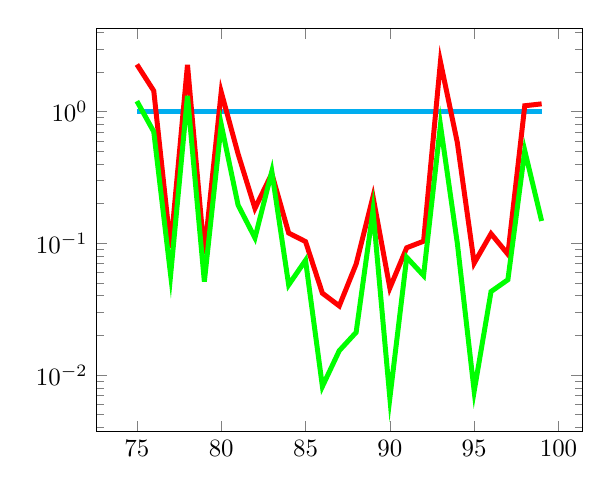
\begin{tikzpicture}[scale=0.9]
\begin{semilogyaxis}
\addplot[color=cyan,line width=2pt,mark options={solid}] coordinates {(75,1.0)(76,1.0)(77,1.0)(78,1.0)(79,1.0)(80,1.0)(81,1.0)(82,1.0)(83,1.0)(84,1.0)(85,1.0)(86,1.0)(87,1.0)(88,1.0)(89,1.0)(90,1.0)(91,1.0)(92,1.0)(93,1.0)(94,1.0)(95,1.0)(96,1.0)(97,1.0)(98,1.0)(99,1.0)};
\addplot[color=red,line width=2pt,mark options={solid}] coordinates {(75,2.2789264582990034)(76,1.438678424849121)(77,0.09235939805573982)(78,2.268568308588588)(79,0.08265023200954366)(80,1.4102295684589745)(81,0.4773397547551119)(82,0.1842126670630519)(83,0.3376004774118298)(84,0.11969327612139664)(85,0.10309374511916654)(86,0.04180725717155975)(87,0.033469494624060465)(88,0.0695549381074493)(89,0.22635944894254595)(90,0.04582381881241599)(91,0.09253852219624549)(92,0.10372958494949941)(93,2.388797363125431)(94,0.5828332056411566)(95,0.07079862924318328)(96,0.11829182236694011)(97,0.08261233372398469)(98,1.1077578950478821)(99,1.14501066537974)};
\addplot[color=green,line width=2pt,mark options={solid}] coordinates {(75,1.2004447557569518)(76,0.7036518303632783)(77,0.05754588771340289)(78,1.31727787997166)(79,0.05122502650704574)(80,0.7992519022739765)(81,0.1952140456828215)(82,0.1099942777813669)(83,0.3508834685181934)(84,0.048357913063476726)(85,0.07430967611376393)(86,0.00819426438889479)(87,0.015302327974158019)(88,0.021081395039292464)(89,0.17731396139660016)(90,0.006687858727171723)(91,0.07825343140228662)(92,0.05693306444192848)(93,0.789135132535879)(94,0.10042428090387144)(95,0.007541911544690249)(96,0.04300385543210978)(97,0.052931193350793895)(98,0.5050409001763532)(99,0.14782404286171422)};

\end{semilogyaxis}
\end{tikzpicture}
